%% Template for MLP Coursework 1 / 19 October 2021 

%% Based on  LaTeX template for ICML 2017 - example_paper.tex at 
%%  https://2017.icml.cc/Conferences/2017/StyleAuthorInstructions

\documentclass{article}
\usepackage[T1]{fontenc}
\usepackage{amssymb,amsmath}
\usepackage{txfonts}
\usepackage{microtype}

% For figures
\usepackage{graphicx}
\usepackage{subcaption} 

% For citations
\usepackage{natbib}

% For algorithms
\usepackage{algorithm}
\usepackage{algorithmic}

% the hyperref package is used to produce hyperlinks in the
% resulting PDF.  If this breaks your system, please commend out the
% following usepackage line and replace \usepackage{mlp2017} with
% \usepackage[nohyperref]{mlp2017} below.
\usepackage{hyperref}
\usepackage{url}
\urlstyle{same}

\usepackage{color}
\usepackage{booktabs} % To thicken table lines
\usepackage{multirow} % Multirow cells in table

% Packages hyperref and algorithmic misbehave sometimes.  We can fix
% this with the following command.
\newcommand{\theHalgorithm}{\arabic{algorithm}}


% Set up MLP coursework style (based on ICML style)
\usepackage{mlp2021}
\mlptitlerunning{MLP Coursework 1 (\studentNumber)}
\bibliographystyle{icml2017}


\DeclareMathOperator{\softmax}{softmax}
\DeclareMathOperator{\sigmoid}{sigmoid}
\DeclareMathOperator{\sgn}{sgn}
\DeclareMathOperator{\relu}{relu}
\DeclareMathOperator{\lrelu}{lrelu}
\DeclareMathOperator{\elu}{elu}
\DeclareMathOperator{\selu}{selu}
\DeclareMathOperator{\maxout}{maxout}



\definecolor{red}{rgb}{0.95,0.4,0.4}
\definecolor{blue}{rgb}{0.4,0.4,0.95}
\definecolor{orange}{rgb}{1, 0.65, 0}

\newcommand{\youranswer}[1]{{\color{red} \bf[#1]}} %your answer: 


%% START of YOUR ANSWERS
%% REPLACE sXXXXXXX with your student number
\def\studentNumber{s2196789}


%% START of YOUR ANSWERS
%% Add answers to the questions below, by replacing the text inside the brackets {} for \youranswer{ "Text to be replaced with your answer." }. 
%
% Do not delete the commands for adding figures and tables. Instead fill in the missing values with your experiment results, and replace the images with your own respective figures.
%
% You can generally delete the placeholder text, such as for example the text "Question Figure 2 - Replace the images ..." 
%
% There are 19 TEXT QUESTIONS (a few of the short first ones have their answers added to both the Introduction and the Abstract). Replace the text inside the brackets of the command \youranswer with your answer to the question.
%
% There are also 3 "questions" to replace some placeholder FIGURES with your own, and 3 "questions" asking you to fill in the missing entries in the TABLES provided. 
%
% NOTE! that questions are ordered by the order of appearance of their answers in the text, and not by the order you should tackle them. Specifically, you cannot answer Questions 2, 3, and 4 before concluding all of the relevant experiments and analysis. Similarly, you should fill in the TABLES and FIGURES before discussing the results presented there. 
%
% NOTE! If for some reason you do not manage to produce results for some FIGURES and TABLES, then you can get partial marks by discussing your expectations of the results in the relevant TEXT QUESTIONS (for example Question 8 makes use of Table 1 and Figure 2).
%
% Please refer to the coursework specification for more details.


%% - - - - - - - - - - - - TEXT QUESTIONS - - - - - - - - - - - - 

%% Question 1:
\newcommand{\questionOne} {
\youranswer{model cannot be well generalized from the original data set to another new data set.}
}

%% Question 2:
\newcommand{\questionTwo} {
\youranswer{will make overfitting worse.}
}

%% Question 3:
\newcommand{\questionThree} {
\youranswer{dropout and L1/L2 regluation will mitigate overfitting problem and improve the performance of the trained model.}
}

%% Question 4:
\newcommand{\questionFour} {
\youranswer{overfitting is an important problem that we need to keep in mind when we train models despite what methods we used}
}

%% Question 5:
\newcommand{\questionFive} {
\youranswer{there is another model $F'$ which makes larger error rate than the given model $F$ on the training example, but the error rate of $F'$'s is smaller than $F$ in the entire distribution.}
}

%% Question 6:
\newcommand{\questionSix} {
\youranswer{There are many reasons that cause the  overfitting, including too much parameters or too high complexity of the model, or overtraining the model.
We can identify it is happening by noticing that the model makes more mistakes on training data but fewer mistakes on unseen future data.}
}

%% Question 7:
\newcommand{\questionSeven} {
\youranswer{it shows the error curve on the training and validation set of EMNIST dataset. The error rate decreases on the training set by going through each epoch. However, the error rate of validation set decreased and reached its minimum at approximately epoch 15, then increases after each epoch. The reason behind this is that our model fits the noise in the training data set which will not re-appear in the validation data set. There is another point which is noticeable. We could find that the slop of error and accuracy curve at first few epoch is steep. It is because at first few epoch the error is large which makes the model learn fast.}
}

%% Question 8:
\newcommand{\questionEight} {
\youranswer{as we increase the hidden units per layer, the generalization gap increases as well. The validation accuracy also increases, but according to the curvature of validation accuracy, even if the model with 128 hidden units(green line) has higher accuracy, it decreases faster after each epoch despite it increasing in the training set, which makes overfitting even worse. We could make a presumption that if we continue train the model with more epoch, the accuracy will become lower than that of 32 or 64 hidden units.}
}

%% Question 9:
\newcommand{\questionNine} {
\youranswer{From above figures we could find out that by adding hidden units up to 64 will kind of increase the validation accuracy, but when we add hidden units up to 128 there will be a dramatic increasing in generalization gap which will make overfitting worse. Hence varying width affects the
does not always results in a consistent way. In the case of 32 hidden units, it might be underfitting for a classifier with 47 different classes. However if there are 128 hidden units, the model becomes overfitting to the training set.}
}

%% Question 10:
\newcommand{\questionTen} {
\youranswer{there is no obvious differences between different depths on training set, but on validation set depth2 has the highest generalization gap. The model with 3 hidden layers has the best performance with highest validation accuracy and smallest generalization gap.}
}

%% Question 11:
\newcommand{\questionEleven} {
\youranswer{The results are not expected or match well with the prior knowledge because increasing depth does not affect the model's performance on training set, and it makes the generalization gap smaller. In other words, it mitigates the overfitting problem. According to prior knowledge, model with too much complexity should be more likely to overfitting to the training set. }
}

%% Question 12:
\newcommand{\questionTwelve} {
\youranswer{By comparing with two figures discussed previously, we could conclude that varying width and height changes the performance and overfitting in different way. If we keeping adding hidden units and make our model more complex, we will get the model overfitting, whereas adding the depth will kind of mitigate overfitting. However, by doing so also makes our model more complex and will get a larger generalization gap than that of model with a single hidden layer and small hidden units(32 and 64), which makes overfitting even worse.}
}

%% Question 13:
\newcommand{\questionThirteen} {
\youranswer{The main idea for L1/L2 regulation is that they aim to control the complexity of our model by adding penalties to loss function and penalize weight. In machine learning, we use gradient descend to train our model. If we add a regulation term to loss function, we make it not differentiable since it has absolute value, which means we add a constrain to loss function. The formula for L1 regulation is
\begin{align}
    L = E_{in}+\lambda\sum_{j}||w_{j}||
\end{align} 
L1 regulation is that it adds a penalty which is equal to the absolute value of the magnitude of coefficient. L1 regulation can produce sparsity, which most of weights in a model are 0. The hyperparameter for L1 regulation is $\lambda$ which controls the magnitude of L1 function. The formula for L2 regulation is
\begin{align}
    L = E_{in}+\lambda\sum_{j}||w_{j}||^{2}
\end{align} 
L2 regulation is that it adds a penalty which is equal to the square of the magnitude of coefficient. L2 regulation can alleviate overfitting. The hyperparameter for L2 regulation is $\lambda$ which performs the same function as in L1 regulation. 
}
}

%% Question 14:
\newcommand{\questionFourteen} {
\youranswer{
Our aim is to minimize loss function when it is constrained regulation. Consider that there are two parameters in weight matrix, $w_1$ and $w_2$. The point which optimized loss function is when the regulation function intersects with the contour of loss function. If we draw a function of L1, it will be a rectangular. Usually the contour of loss function will touch the L1 function at a corner, leading a sparsity solution. The function of L2 regulation is circular. We will always get small parameters(but nonzero) for weight when the contour of loss function touches the L2 function. Small parameters will make our model robust because they can fit in various data set. Large parameters are sensitive to various data set. In summary, both L1 and L2 regulation can address overfitting.
}
}

%% Question 15:
\newcommand{\questionFifteen} {
\youranswer{By comparing the validation accuracy and generalization gap of the baseline model and regularized models, we could find that the models implemented with dropout layer or L1/L2 penalty have higher validation accuracy and smaller generalization gap. Adjusting hyperparameter values also changes the performance of the model. In figure 4, it shows that the model has the best performance when the dropout value ranges between 0.4 and 0.6. And for weight decay value, the model performs poorly when the weight decay value is too large($10^-2$ or $10^-1$). We got the best overall results when L2 regulation was implemented individually. Its validation accuracy and generalization gap are obviously better than previous model which does not have overfitting problem. In combination of dropout and L1/L2 regulation, we found that implements dropout layers together with L1/L2 regulation does not improve the model's performance. To explain this phenomena, according to the function of L1/L2 regulation, we could assume that the weights in model with L1/L2 regulation are already regularized not to overfit the training set. If we drop out some weights based on this, it could decrease the accuracy of the model, but the generalization performance of the model is still good since it does not have overfiting problem. 
}
}

%% Question 16:
\newcommand{\questionSixteen} {
\youranswer{it can't fit well with ideal stochastic gradient operation and its approximation for the deep model could be enhanced}

}

%% Question 17:
\newcommand{\questionSeventeen} {
\youranswer{Dropout is compitable with Maxout activation function because Maxout  is locally linear. Unlike other activation functions such as ReLU or sigmoid, which constraints dropout model averaging, Maxout has better performance when trained with dropout by its property of piecewise linear function.
}
}

%% Question 18:
\newcommand{\questionEighteen} {
\youranswer{In the experiment the authors evaluated the Maxout model by testing it with four different dataset, MNIST, CIFAR-10, CIFAR-100, and SVHN, and comparing the test results with that of other methods. They conclude that the Maxout model together with dropout has the lowest test error. In addition, they also point out that the enhancement of test error is not from preprocessing or large models, but from the use of Maxout. The authors compare Maxout to rectifiers with the same processing by a set of cross-validation experiments and they find Maxout performs better than rectifiers}
}

%% Question 19:
\newcommand{\questionNineteen} {
\youranswer{Based on the results from reviewing of Maxout networks, we found that although Maxout can improve accuracy and minimize error for dropout, it may also cause overfitting problem in some extreme cases. Maxout is not always the best choice over other methods. In machine learning there are many complicated circumstances in which data are usually complex and unexpected. There are many methods we could use to mitigating overfitting such as dropout, L1/L2 regulation, but we need to pay attention to this problem because it happens frequently when we train models despite what methods we used}
}


%% - - - - - - - - - - - - FIGURES - - - - - - - - - - - - 

%% Question Figure 2:
\newcommand{\questionFigureTwo} {


\begin{figure}[t]
    \centering
    \begin{subfigure}{\linewidth}
        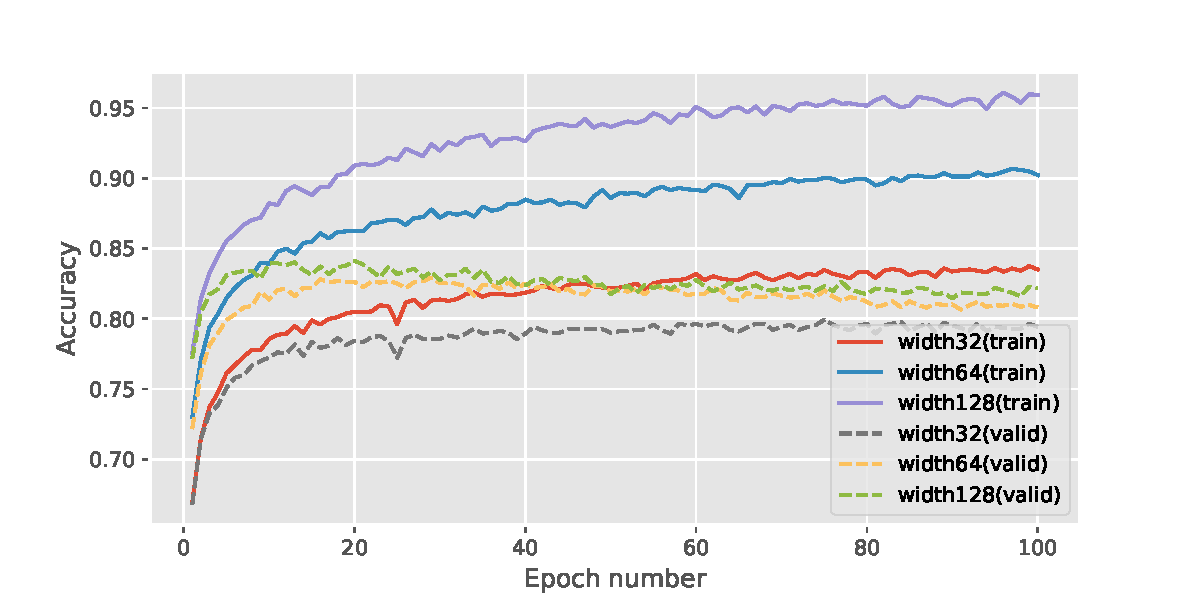
\includegraphics[width=\linewidth]{hidden_unit_acc.pdf}
        \caption{accuracy by epoch}
        \label{fig:width_acccurves}
    \end{subfigure} 
    \begin{subfigure}{\linewidth}
        \centering
        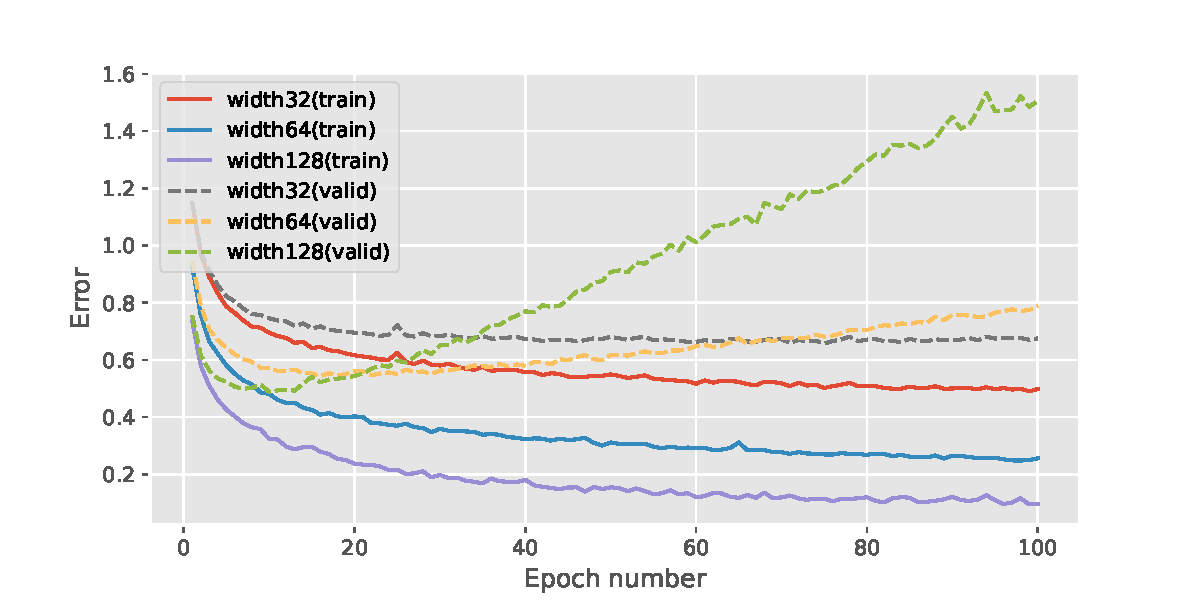
\includegraphics[width=\linewidth]{hidden_unit_err.pdf}
        \caption{error by epoch}
        \label{fig:width_errorcurves}
    \end{subfigure} 
    \caption{Training and validation curves in terms of classification accuracy (a) and cross-entropy error (b) on the EMNIST dataset for different network widths.}
    \label{fig:width}
\end{figure} 


}

%% Question Figure 3:
\newcommand{\questionFigureThree} {


\begin{figure}[t]
    \centering
    \begin{subfigure}{\linewidth}
        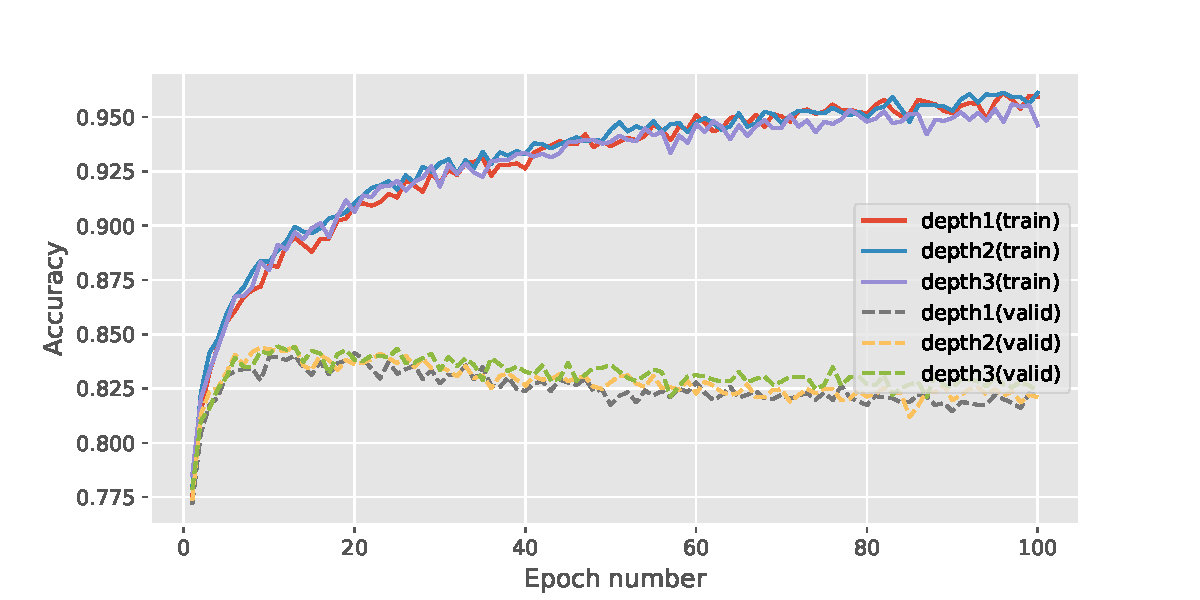
\includegraphics[width=\linewidth]{hidden_layer_acc.pdf}
        \caption{accuracy by epoch}
        \label{fig:depth_acccurves}
    \end{subfigure} 
    \begin{subfigure}{\linewidth}
        \centering
        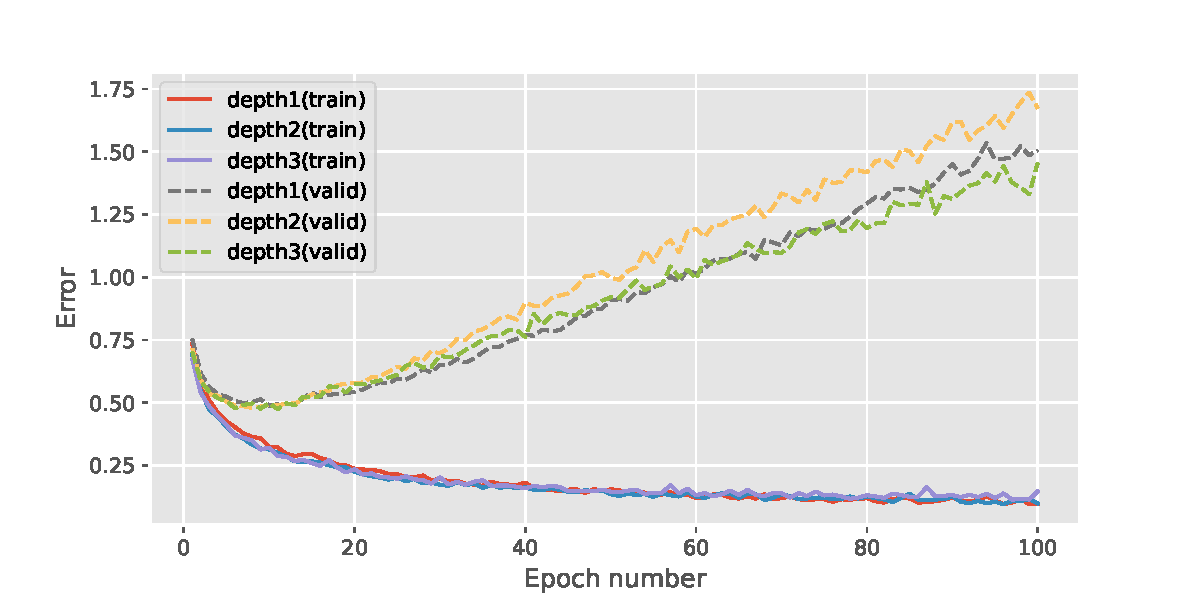
\includegraphics[width=\linewidth]{hidden_layer_err.pdf}
        \caption{error by epoch}
        \label{fig:depth_errorcurves}
    \end{subfigure} 
    \caption{Training and validation curves in terms of classification accuracy (a) and cross-entropy error (b) on the EMNIST dataset for different network depths.}
    \label{fig:depth}
\end{figure} 


}

%% Question Figure 4:
\newcommand{\questionFigureFour} {

\begin{figure*}[t]
    \centering
    \begin{subfigure}{.49\linewidth}
        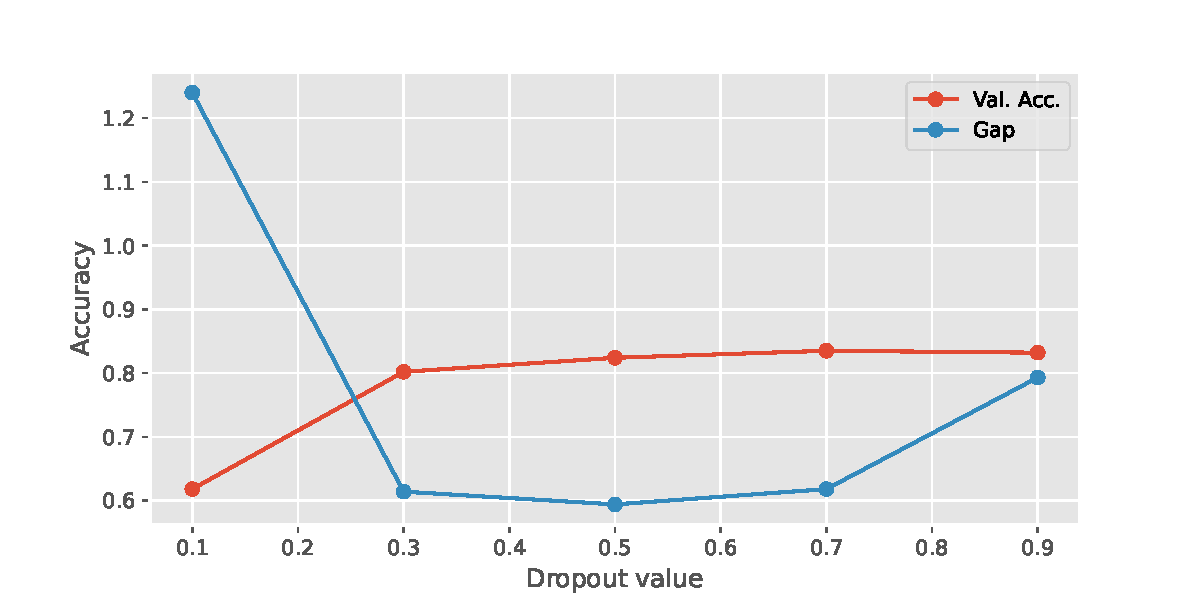
\includegraphics[width=\linewidth]{dropout.pdf}
        \caption{Metrics by dropout rate}
        \label{fig:dropoutrates}
    \end{subfigure} 
    \begin{subfigure}{.49\linewidth}
        \centering
        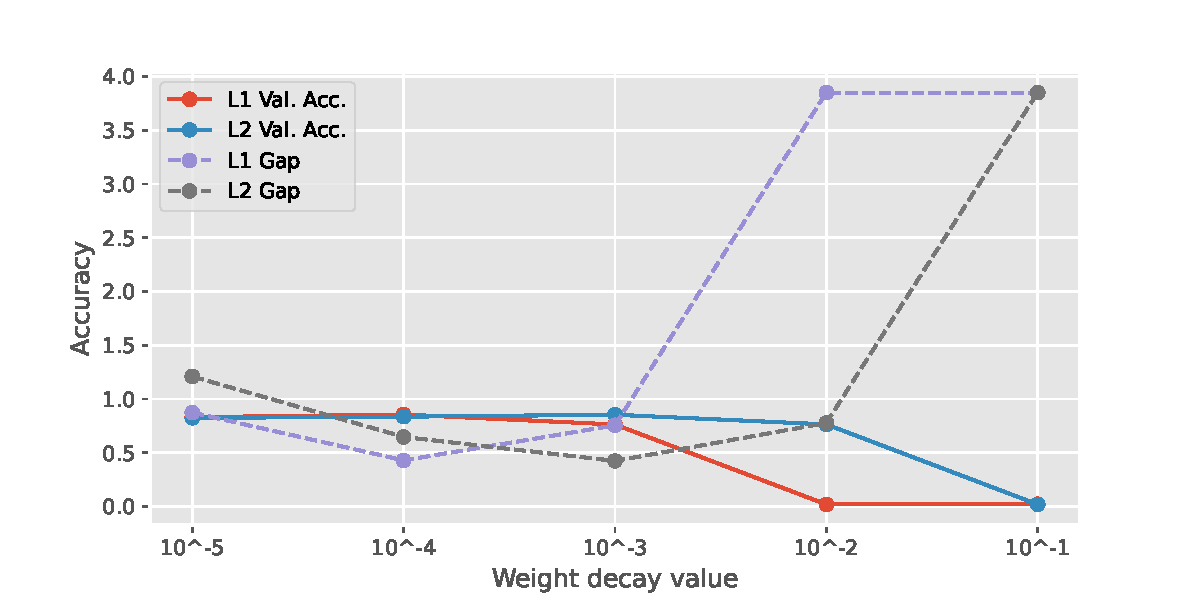
\includegraphics[width=\linewidth]{weightdecay.pdf}
        \caption{Metrics by weight penalty}
        \label{fig:weightrates}
    \end{subfigure} 
    \begin{subfigure}{\linewidth}
        \centering
        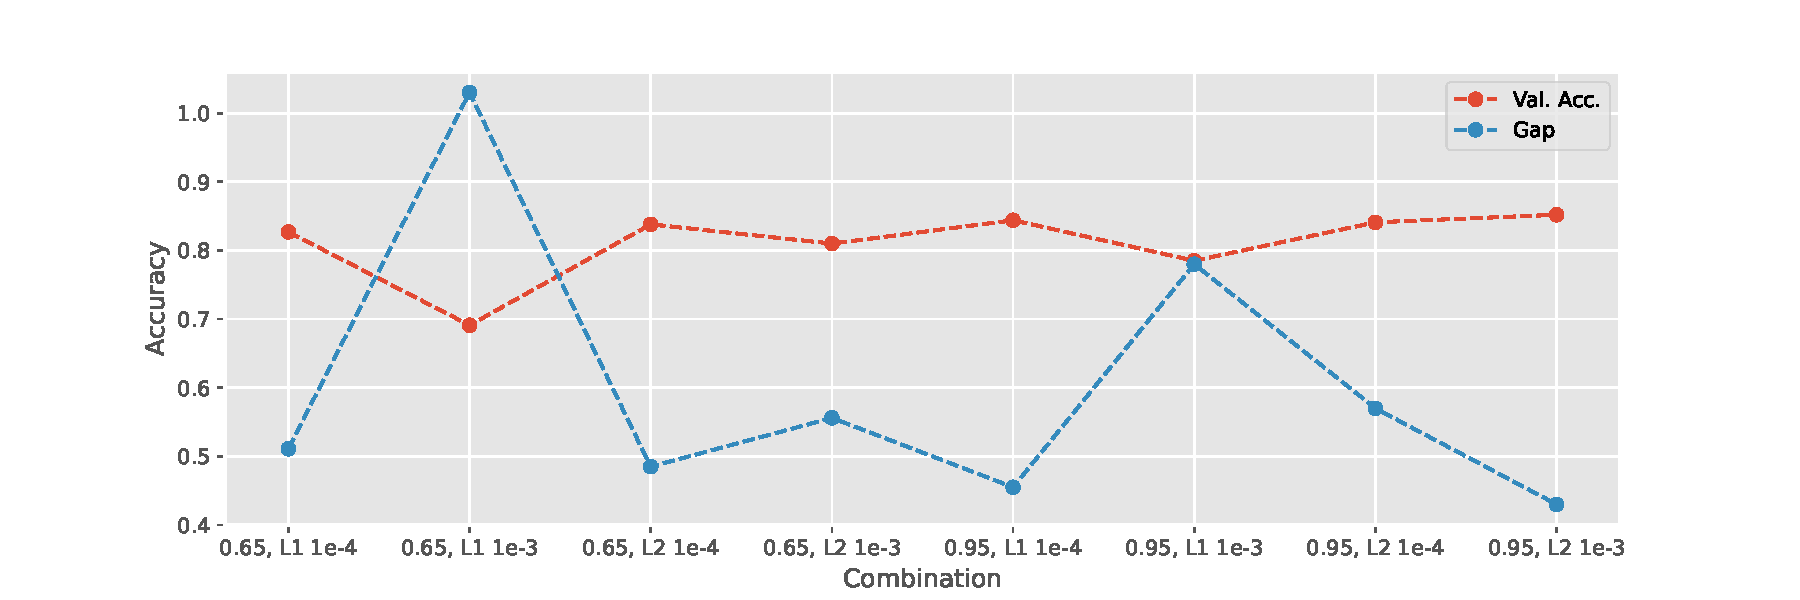
\includegraphics[width=\linewidth]{combination.pdf}
        \caption{Extra experiments}
        \label{fig:extra}
    \end{subfigure} 
    \caption{Hyperparameter search for every method and combinations}
    \label{fig:hp_search}
\end{figure*}


}

%% - - - - - - - - - - - - TABLES - - - - - - - - - - - - 

%% Question Table 1:

\newcommand{\questionTableOne} {


\begin{table}[t]
    \centering
    \begin{tabular}{c|cc}
    \toprule
        \# hidden units & val. acc. & generalization gap \\
    \midrule
         32       &     0.798        &    0.658                    \\
         64       &     0.813         &   0.768                    \\
         128      &     0.815        &    1.55                   \\ 
    \bottomrule
    \end{tabular}
    \caption{Validation accuracy (\%) and generalization gap (in terms of cross-entropy error) for varying network widths on the EMNIST dataset.}
    \label{tab:width_exp}
\end{table}
}


%% Question Table 2:
\newcommand{\questionTableTwo} {


\begin{table}[t]
    \centering
    \begin{tabular}{c|cc}
    \toprule
        \# hidden layers & val. acc. & generalization gap \\
    \midrule
         1          &     0.815       &     1.55                    \\
         2         &      0.818        &    1.73                    \\
         3               &      0.821      &    1.45                \\ 
    \bottomrule
    \end{tabular}
    \caption{Validation accuracy (\%) and generalization gap (in terms of cross-entropy error) for varying network depths on the EMNIST dataset.}
    \label{tab:depth_exps}
\end{table}

}

%% Question Table 3:
\newcommand{\questionTableThree} {


\begin{table*}[t]
    \centering
    \begin{tabular}{c|c|cc}
    \toprule
        Model    &  Hyperparameter value(s) & Validation accuracy & Generalization gap \\
    \midrule
    \midrule
        Baseline &  -                    &         0.821            &          1.45         \\
    \midrule
        \multirow{5}*{Dropout}
                 & 0.1                   &         0.618            &          1.24         \\
                 & 0.3                   &          0.802           &         0.614          \\
                 & 0.5                   &          0.824           &         0.594          \\
                 & \emph{0.7}            &      \emph{0.835}        &     \emph{0.618}       \\
                 & 0.9                   &          0.832           &         0.793          \\
    \midrule
        \multirow{5}*{L1 penalty}
                 & 1e-5                   &        0.831             &       0.874            \\
                 & \emph{1e-4}            &    \emph{0.855}          &   \emph{0.429}          \\
                 & 1e-3                   &        0.763             &       0.756            \\
                 & 1e-2                   &        0.020             &       3.850            \\
                 & 1e-1                   &        0.022             &       3.850            \\
    \midrule
        \multirow{5}*{L2 penalty}  
                 & 1e-5                   &       0.825              &      1.21             \\
                 & 1e-4                   &       0.836              &      0.647             \\
                 & \textbf{1e-3}            &   \textbf{0.854}           &  \textbf{0.424}          \\
                 & 1e-2                   &       0.764              &      0.778             \\
                 & 1e-1                   &       0.020              &      3.85             \\
    \midrule
        \multirow{8}*{Combined}  
                 & 0.65, L1 1e-4                 &         0.827            &       0.511            \\
                 & 0.65, L1 1e-3                 &          0.691           &       1.03            \\
                 & 0.65, L2 1e-4                   &        0.838             &     0.485              \\
                 & 0.65, L2 1e-3                  &         0.81            &       0.556            \\
                 &\emph{0.95, L1 1e-4}           &      \emph{0.844}        &    \emph{0.455}          \\
                 & 0.95, L1 1e-3                  &         0.758            &      0.78             \\
                 & 0.95, L2 1e-4                  &         0.841            &      0.570             \\
                 & 0.95, L2 1e-3                  &        0.852             &       0.430            \\
    \bottomrule
    \end{tabular}
    \caption{Results of all hyperparameter search experiments. \emph{italics} indicate the best results per series and \textbf{bold} indicate the best overall}
    \label{tab:hp_search}
\end{table*}


}

%% END of YOUR ANSWERS
%% END of YOUR ANSWERS



%% Do not change anything in this file. Add your answers to mlp-cw1-questions.tex



\begin{document} 

\twocolumn[
\mlptitle{MLP Coursework 1}
\centerline{\studentNumber}
\vskip 7mm
]

\begin{abstract} 
In this report we study the problem of overfitting, which is \questionOne.
We first analyse the given example and discuss the probable causes of the underlying problem. 
Then we investigate how the depth and width of a neural network
can affect overfitting in a feedforward architecture and observe that increasing width and depth \questionTwo.
Next we discuss why two standard methods, Dropout and Weight Penalty, can
mitigate overfitting, then describe their implementation and use them in our experiments
to reduce the overfitting on the EMNIST dataset. 
Based on our results, we ultimately find that \questionThree.
Finally, we briefly review another method, Maxout, discuss its strengths and weaknesses, and conclude the report with our observations and future work. Our main findings indicate that \questionFour.
\end{abstract} 

\section{Introduction}
\label{sec:intro}
In this report we focus on a common and important problem while training machine learning models known as overfitting, or overtraining, which is \questionOne.
We first start with analyzing the given problem in Fig.~\ref{fig:example}, study it in different architectures and then investigate different strategies to mitigate the problem.
In particular, Section \ref{sec:task1} identifies and discusses the given problem, and investigates the effect of network width and depth in terms of generalization gap (see Ch.~5 in \citealt{Goodfellow-et-al-2016}) and generalization performance.
Section \ref{sec:task2.1} introduces two regularization techniques to alleviate overfitting: Dropout \cite{srivastava2014dropout} and L1/L2 Weight Penalties (see Section~7.1 in \citealt{Goodfellow-et-al-2016}). 
We first explain them in detail and discuss why they are used for alleviating overfitting.
In Section~\ref{sec:task2.2} we incorporate each of them and their various combinations to a three hidden layer neural network, train it on the EMNIST dataset, which contains 131,600 images of characters and digits, each of size 28x28 which are split into 47 classes, grouping together some difficult to distinguish characters.
We evaluate them in terms of generalization gap and performance, and discuss the results and effectiveness of the tested regularization strategies.
Our results show that \questionThree.
In Section~\ref{sec:task3}, we discuss a related work on Maxout Networks and highlight its pros and cons.\footnote{Instructor note: Omitting this for this coursework, but normally you would be more specific and summarise your conclusions about that review here as well.}
Finally, we conclude our study in section \ref{sec:concl}, noting that \questionFour.


\section{Problem identification}
\label{sec:task1}

\begin{figure}[t]
    \centering
    \begin{subfigure}{\linewidth}
        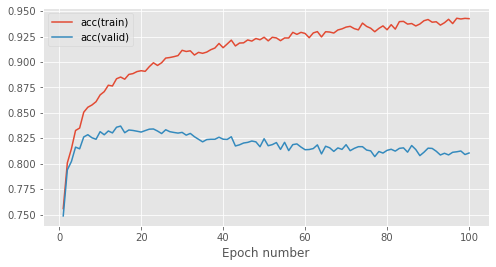
\includegraphics[width=\linewidth]{accuracy_IHO_withrelu.png}
        \caption{accuracy by epoch}
        \label{fig:example_acccurves}
    \end{subfigure} 
    \begin{subfigure}{\linewidth}
        \centering
        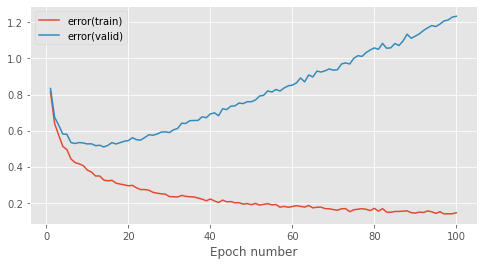
\includegraphics[width=\linewidth]{error_IHO_withrelu.png}
        \caption{error by epoch}
        \label{fig:example_errorcurves}
    \end{subfigure} 
    \caption{Training and validation curves in terms of classification accuracy (a) and cross-entropy error (b) on the EMNIST dataset for the baseline model.}
    \label{fig:example}
\end{figure} 

Overfitting to training data is a very common and important issue that needs to be dealt with when training neural networks or other machine learning models in general (see Ch.~5 in \citealt{Goodfellow-et-al-2016}).
A model is said to be overfitting when \questionFive.

\questionSix.

Fig.~\ref{fig:example_acccurves} and \ref{fig:example_errorcurves} show a prototypical example of overfitting.
We see in Figure~\ref{fig:example_acccurves} that \questionSeven.

The extent to which our model overfits depends on many factors.
For example, the quality and quantity of the training set and
the complexity of the model. If we have a lot of varied training samples,
or if our model is relatively shallow, it will in general
be less prone to overfitting. Any form of regularisation
will also limit the extent to which the model overfits.


\subsection{Network width}

\questionTableOne
\questionFigureTwo


First we investigate the effect of increasing the number of
hidden units in a single hidden layer network when training
on the EMNIST dataset.
The network is trained using the Adam optimizer
with a learning rate of $10^{-3}$ and a batch size of 100, for a total of 100 epochs.


The input layer is of size 784, and output layer consists
of 47 units. 
Three different models were trained, with a
single hidden layer of 32, 64 and 128 ReLU hidden units
respectively.
Figure~\ref{fig:width} depicts the error and accuracy curves over 100 epochs for the model with varying number of hidden units.
Table~\ref{tab:width_exp} reports the final accuracy and generalization gap.
We observe that \questionEight.

\questionNine.


\subsection{Network depth}

\questionTableTwo
\questionFigureThree

Next we investigate the effect of varying the number of hidden
layers in the network. 
Table~\ref{tab:depth_exps} and Fig.~\ref{fig:depth} shows the results from
training three models with one, two and three hidden layers respectively,
each with 128 ReLU hidden units. 
As with previous experiments, they are 
trained with the Adam optimizer with a learning rate of  $10^{-3}$ and 
a batch size of 100. 

We observe that \questionTen.

\questionEleven.

\questionTwelve.





\section{Dropout and Weight Penalty}
\label{sec:task2.1} 

In this section, we investigate three regularization methods to 
alleviate the overfitting problem, specifically dropout layers 
and the L1 and L2 weight penalties.

\subsection{Dropout}

Dropout~\cite{srivastava2014dropout}
is a stochastic method that randomly inactivates
neurons in a neural network according to an hyperparameter, the
dropout rate. Dropout is commonly represented by an 
additional layer inserted between the linear layer and 
activation function.
Its forward propagation during training is defined as follows:

\begin{align}
    mask &\sim bernoulli(p)\\
    y' &= mask \odot y\
\end{align}

where $y, y' \in \mathbb{R}^d$ are the output of the linear layer 
before and after applying dropout, 
respectively. $mask \in \mathbb{R}^d$ is a mask vector randomly sampled from the
Bernoulli distribution with parameter of inclusion probability
$p$, and $\odot$ denotes the element-wise multiplication.

At inference time, stochasticity is not desired, so no neurons
are dropped. To account for the change in expectations of the
output values, we scale them down by the inclusion rate
$p$:

\begin{align}
    y' &= y*p\
\end{align}

As there is no nonlinear calculation involved, the backward
propagation is just the element-wise product of the gradients
with respect to the layer outputs and mask created
in the forward calculation. The backward propagation for
dropout is therefore formulated as follows:

\begin{align}
    \frac{\partial y'}{\partial y} = mask
\end{align}

Dropout is an easy to implement and highly scalable
method. It can be implemented as a layer-based calculation
unit, and be placed on any layer of the neural network at
will. Dropout can reduce the dependence of hidden features
between layers so that the neurons of the next layer will not
specifically depend on some features from of the previous layer.
Instead, it force the network to evenly distribute information
among all features. By randomly dropping some neurons in training,
dropout makes use of a subset of the whole architecture, so it can 
also be viewed as bagging different sub networks and averaging their
outputs.



\subsection{Weight penalty}

L1 and L2 regularization~\cite{ng2004feature} are simple but effective
methods to mitigate overfitting to training data.
\questionThirteen.

\questionFourteen.



\section{Balanced EMNIST Experiments}

\questionTableThree

\questionFigureFour

\label{sec:task2.2}

Here we evaluate the effectiveness of the given regularization methods for reducing the overfitting on the EMNIST dataset.
We build a baseline architecture with three hidden layers, each with 128 neurons, which suffers from overfitting in EMNIST as shown in section \ref{sec:task1}.
We follow the previous training settings where we deliberately let the baseline overfit
on the training set as in previous experiments. 
These settings ensure the fairness of the evaluation of three methods to alleviate overfitting. 
Then, we apply the L1 or L2 regularization with dropout to our baseline and search for good hyperparameters on the validation set. 
We summarize all
the experimental results in Table~\ref{tab:hp_search}. For each method, we
plot the relationship between generalisation gap and validation accuracy in Figure~\ref{fig:hp_search}.

First we analyze three methods separately, train each over a set of hyperparameters and compare their best performing results.

\questionFifteen.


\section{Literature Review: Maxout Networks}
\label{sec:task3}

\paragraph{Summary of Maxout Networks} In this section, we
briefly discuss another generalization method: Maxout net-
works \cite{goodfellow2013maxout}. This paper further ex-
plores the dropout method and proposes a new "maxout" layer
 which can complement dropout.
The authors evaluate the performance of Maxout Networks
in four standard datasets, namely MNIST, CIFAR-10
and 100, and SVHN. They point out that although
dropout has been widely applied in deep models, \questionSixteen. Following this 
motivation, they propose the Maxout activation layers. These can be considered learnable activations that work as a universal convex function approximator. The Maxout layer first
maps the hidden space to $k$ subspaces through independent
affine transformations, then, for each element in output
vectors, it takes the maximum value across all subspaces.

\questionSeventeen.

\paragraph{Strengths and limitations} The author proposed a novel
neural activation unit that further exploits the dropout technique.
\questionEighteen.

Although the Maxout activation units can maximize
the averaging effect of dropout in a deep architecture,
we can argue that the Maxout computation
is expensive. The advantage of dropout lies in its high 
scalability and computational advantages. It can be arbitrarily
applied to various network structures, and the calculation
speed is fast, which is very suitable for heavy computing 
algorithms such as training and inference of neural networks.
In comparison, the design of the Maxout network needs to project the
hidden vector into $k$ subspaces. Both the forward algorithm and the
backward algorithm of dropout can be calculated in $\mathcal{O}(D)$
complexity, but the complexity of Maxout is $\mathcal{O}(kD)$.
This can lead to increasing the number of training epochs needed
to reach convergence. 
Furthermore, the universal approximation property of Maxout seems
powerful, but it would be interesting to verify that it is useful
in practice. Specifically, we can design an experiment where we 
increase the number of subspaces $k$ and see where performances stop
improving. In extreme cases, it is even possible that the 
function learned is too specific to the training data, effectively
causing overfitting.



\section{Conclusion}
\label{sec:concl}
    
\questionNineteen.

\bibliography{refs}

\end{document} 

